\documentclass[journal]{IEEEtran}

\usepackage{amsmath,amssymb}
\usepackage{booktabs}
\usepackage{graphicx}
\usepackage{microtype}
\usepackage[hidelinks]{hyperref}
\usepackage{xspace}

\graphicspath{{figures/}}
\hypersetup{pdfauthor={Amir Ghorbani},pdftitle={Supplementary Material for TRACE-R}}
\newcommand{\tracer}{TRACE-R\xspace}

\begin{document}

\title{Supplementary Material for ``TRACE-R: Telemetry-Routed Adaptive Corruption-Expert Restoration for Pavement Inspection''}
\author{Amir~Ghorbani}
\maketitle

\section{Capture Interface}
The public packet contains 82 normalized values. Entries 1--33 are eleven three-axis gyroscope samples and entries 34--66 are eleven three-axis accelerometer samples, both centred on exposure. The remaining context entries are, in order: log exposure, log ISO, analog gain, focal length, aperture, focus-error proxy, autofocus confidence, rolling-shutter readout, vehicle speed, vehicle yaw rate, timestamp offset, IMU noise, camera reliability, IMU reliability, vehicle reliability, and global availability. Camera, IMU, and vehicle masks are independent.

The deterministic map is implemented by \texttt{observable\_code\_from\_packet}. The reported router is implemented by \texttt{TRACERExpertFusion.route}. Neither function accepts a dataset identifier, scenario label, target image, detector label, or hidden synthetic kernel. Controlled sidecars use the same packet order as measured KITTI and CRID records.

\begin{table}[!t]
\centering
\caption{Validation-fixed TRACE-R routing constants.}
\label{tab:route_constants}
\footnotesize
\begin{tabular}{lr}
\toprule
Quantity & Value \\
\midrule
Motion threshold $t_M$ & 0.180 \\
Defocus threshold $t_D$ & 0.200 \\
Low-light threshold $t_L$ & 0.385 \\
Reliability threshold $q_0$ & 0.500 \\
DFPIR weight, low-light route & 0.400 \\
DFPIR weight, mixed route & 0.075 \\
Gyroscope full scale & 4.0 \\
\bottomrule
\end{tabular}
\end{table}

Motion uses DFPIR and defocus uses InstructIR. The low-light blend is $0.40$ DFPIR plus $0.60$ DeMoE; the mixed blend is $0.075$ DFPIR plus $0.925$ DeMoE. The all-unavailable route uses DeMoE. These coefficients are stored by \texttt{TRACERPolicy}; they are not recomputed for an evaluation image.

\section{Matched Adaptation and Checkpoints}
Every controlled restorer receives 70 total target-domain epochs, 4,096 effective optimizer updates, an effective batch size of four, and source-balanced IVCNZ/PCM sampling. AdamW uses an initial learning rate of $10^{-5}$ and weight decay $10^{-4}$. The common objective has Charbonnier coefficient 1.0, gradient coefficient 0.15, frozen-detector feature coefficient 0.20, and frozen supervised detector coefficient 0.10. Detector features are taken from layers \texttt{model.2} and \texttt{model.4} with relative weights 0.5 and 1.0. Detector terms use a one-epoch linear warm-up. Validation mAP50 selects checkpoints; the training script does not evaluate a test split.

\begin{table*}[!t]
\centering
\caption{Matched target-domain adaptation and selection budget.}
\label{tab:training_audit}
\footnotesize
\setlength{\tabcolsep}{3.7pt}
\begin{tabular}{lrrl}
\toprule
Method & Epochs & Optimizer steps & Selection endpoint \\
\midrule
NAFNet & 70 & 4,096 & joint validation mAP50 \\
FiLM-NAFNet & 70 & 4,096 & joint validation mAP50 \\
InstructIR & 70 & 4,096 & joint validation mAP50 \\
DFPIR & 70 & 4,096 & joint validation mAP50 \\
DeMoE & 70 & 4,096 & joint validation mAP50 \\
TRACE-R router & matched experts & 0 & joint validation mAP50 \\
\bottomrule
\end{tabular}
\end{table*}


\begin{table}[!t]
\centering
\caption{TRACE-R expert checkpoints.}
\label{tab:checkpoints}
\footnotesize
\setlength{\tabcolsep}{3.7pt}
\begin{tabular}{lrl}
\toprule
Expert & Adaptation epochs & SHA-256 prefix \\
\midrule
DeMoE & 70 & \texttt{743f106d380bd8db} \\
DFPIR & 70 & \texttt{cca8f4b00a2e6468} \\
InstructIR & 70 & \texttt{4d97860f360bf21c} \\
\bottomrule
\end{tabular}
\end{table}


TRACE-R does not receive an additional optimization budget. It composes the selected DFPIR, InstructIR, and DeMoE checkpoints in Table~\ref{tab:checkpoints}. NAFNet and FiLM-NAFNet are trained under the same common objective but are not included in the expert bank because their validation accuracy is lower.

\section{Controlled Results}
Table~\ref{tab:condition_results} gives all eight controlled condition results. TRACE-R wins or ties seven conditions. DeMoE is higher on PCM mixed degradation by 0.0006 before rounding. This exception is retained in the ledger and is not rounded into a strict TRACE-R win.

\begin{table*}[!t]
\centering
\caption{Condition-level mAP50 on IVCNZ and PCM.}
\label{tab:condition_results}
\footnotesize
\setlength{\tabcolsep}{3.7pt}
\begin{tabular}{lrrrrrrrr}
\toprule
Method & \multicolumn{4}{c}{IVCNZ} & \multicolumn{4}{c}{PCM} \\
\cmidrule(lr){2-5}\cmidrule(lr){6-9}
& Mot. & Def. & Low & Mix. & Mot. & Def. & Low & Mix. \\
\midrule
NAFNet & 0.374 & 0.297 & 0.542 & 0.385 & 0.169 & 0.142 & 0.212 & 0.039 \\
FiLM-NAFNet & 0.375 & 0.296 & 0.544 & 0.387 & 0.170 & 0.146 & 0.221 & 0.047 \\
InstructIR & 0.510 & \textbf{0.523} & 0.546 & 0.433 & 0.316 & 0.297 & 0.267 & 0.081 \\
DFPIR & \textbf{0.543} & 0.498 & \textbf{0.555} & 0.415 & \textbf{0.345} & \textbf{0.302} & 0.296 & 0.138 \\
DeMoE & 0.536 & 0.509 & 0.543 & 0.480 & 0.326 & 0.289 & 0.308 & \textbf{0.212} \\
TRACE-R & \textbf{0.543} & \textbf{0.523} & 0.553 & \textbf{0.482} & \textbf{0.345} & 0.297 & \textbf{0.311} & 0.211 \\
\bottomrule
\end{tabular}
\end{table*}


\begin{table*}[!t]
\centering
\caption{Paired fidelity over all four controlled conditions.}
\label{tab:fidelity}
\footnotesize
\setlength{\tabcolsep}{3.7pt}
\begin{tabular}{lrrrr}
\toprule
Method & \multicolumn{2}{c}{IVCNZ} & \multicolumn{2}{c}{PCM} \\
\cmidrule(lr){2-3}\cmidrule(lr){4-5}
& PSNR & SSIM & PSNR & SSIM \\
\midrule
Degraded input & 16.70 & 0.472 & 18.23 & 0.613 \\
InstructIR & 21.20 & 0.656 & 24.52 & 0.807 \\
DFPIR & 24.06 & 0.707 & 26.32 & 0.826 \\
DeMoE & 23.78 & 0.715 & 26.13 & 0.838 \\
TRACE-R & 24.12 & 0.726 & 26.46 & 0.842 \\
\bottomrule
\end{tabular}
\end{table*}


\begin{table}[!t]
\centering
\caption{TRACE-R packet interventions.}
\label{tab:metadata_controls}
\footnotesize
\setlength{\tabcolsep}{3.7pt}
\begin{tabular}{lrrr}
\toprule
Packet supplied at inference & IVCNZ & PCM & Joint \\
\midrule
Aligned packet & 0.525 & 0.291 & 0.408 \\
All sensor groups unavailable & 0.466 & 0.236 & 0.351 \\
Wrong-condition packet & 0.451 & 0.213 & 0.332 \\
\bottomrule
\end{tabular}
\end{table}


Figure~\ref{fig:ivcnz_supp} is the complete IVCNZ comparison used in the main paper. TRACE-R and DeMoE tie on recovered ground-truth count for this frame. The example is retained because it was selected by the fixed recovery rule and illustrates the aggregate low-light behavior without implying a strict image-level win.

\begin{figure*}[!t]
\centering
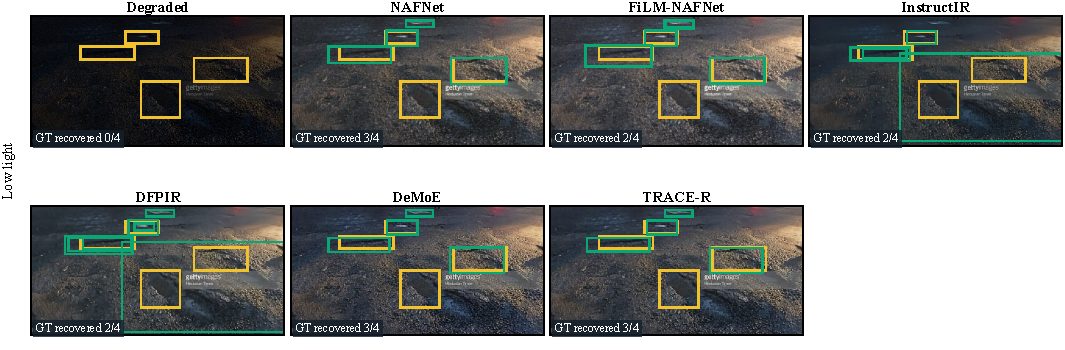
\includegraphics[width=\textwidth]{fig_trace_ivcnz_qualitative.pdf}
\caption{IVCNZ validation example with all controlled comparators. Yellow: annotation; green: detector prediction.}
\label{fig:ivcnz_supp}
\end{figure*}

\section{Measured KITTI Transfer}
The KITTI study uses drive-disjoint images and measured OXTS motion. Its checkpoint belongs to the earlier RMR-P arXiv model; it is not presented as a TRACE-R expert-router result. The purpose is to verify that the 82-value interface can be populated from a public measured motion record.

\begin{table}[!t]
\centering
\caption{Drive-disjoint KITTI transfer with measured OXTS telemetry.}
\label{tab:kitti_supp}
\footnotesize
\begin{tabular}{llrrr}
\toprule
Method & Capture input & PSNR & SSIM & $\Delta$PSNR \\
\midrule
Degraded input & none & 26.06 & 0.845 & 0.00 \\
NAFNet & none & 26.03 & 0.848 & -0.03 \\
FiLM-NAFNet & OXTS & 25.96 & 0.846 & -0.10 \\
RMR-P & unavailable packet & 26.82 & 0.865 & +0.76 \\
RMR-P & OXTS & \textbf{26.86} & \textbf{0.865} & \textbf{+0.79} \\
\bottomrule
\end{tabular}
\end{table}

\begin{figure*}[!t]
\centering
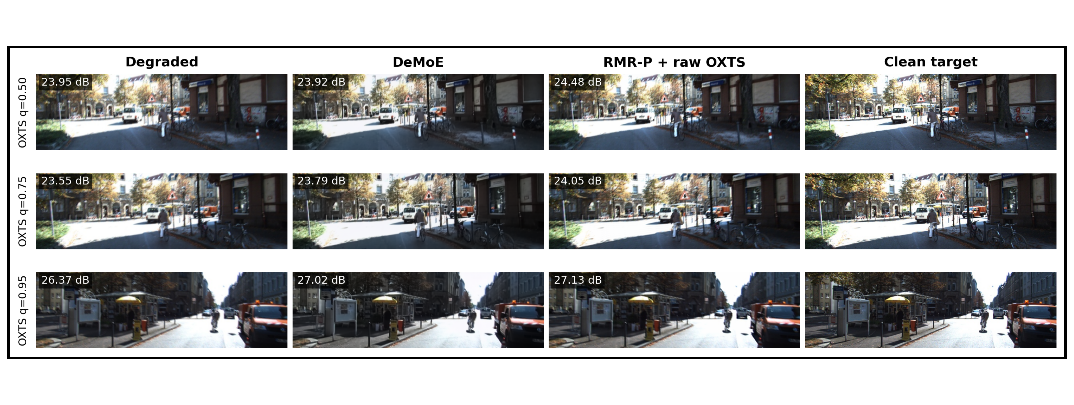
\includegraphics[width=\textwidth]{fig_trace_kitti_qualitative.pdf}
\caption{Drive-disjoint KITTI paired transfer. The panel preserves the executed RMR-P checkpoint name.}
\label{fig:kitti_supp}
\end{figure*}

\section{CRID Field Protocol}
CRID images remain at $4752\times3168$. No synthetic degradation is added. The restoration expert is adapted on unlabelled CRID imagery and paired synthetic corruptions without reading the 46 manual field labels. The detector and policy operate at native image coordinates.

The earlier 12-frame temporal segment fixes the complete field policy in Table~\ref{tab:crid_policy}. The evidence statistic is the sum of squared detector confidences above 0.05. A zero relative margin admits restored evidence only when its score is strictly higher than the native score. Restored predictions below 0.10 are omitted before same-family fusion, and duplicates are removed at IoU 0.15. The detector operating threshold is 0.20. These are the exact values in \texttt{frozen\_policy\_before\_supportive\_test.json}.

\begin{table}[!t]
\centering
\caption{Frozen CRID detector-evidence policy.}
\label{tab:crid_policy}
\footnotesize
\begin{tabular}{lr}
\toprule
Quantity & Value \\
\midrule
Evidence statistic & $\sum_{p_i\ge0.05}p_i^2$ \\
Relative gate margin $\tau$ & 0.000 \\
Restored-prediction floor & 0.100 \\
Same-family fusion IoU & 0.150 \\
Detector operating threshold & 0.200 \\
\bottomrule
\end{tabular}
\end{table}

The subsequent 13-frame temporal block contains 49 ground-truth objects. Table~\ref{tab:crid} repeats the complete ranked comparison. The block was inspected during prior development and is therefore supportive rather than newly sealed evidence.

\begin{table*}[!t]
\centering
\caption{CRID native-image detection on the 13-frame temporal evaluation block.}
\label{tab:crid}
\footnotesize
\setlength{\tabcolsep}{3.7pt}
\begin{tabular}{lrrr}
\toprule
Input & AP@.10 & AP@.50 & Mean \\
\midrule
Raw image & 0.516 & 0.446 & 0.481 \\
NAFNet & 0.559 & 0.474 & 0.516 \\
DFPIR & 0.550 & 0.452 & 0.501 \\
DeMoE & 0.551 & 0.452 & 0.502 \\
InstructIR & 0.542 & 0.442 & 0.492 \\
TRACE-R & \textbf{0.560} & \textbf{0.484} & \textbf{0.522} \\
\bottomrule
\end{tabular}
\end{table*}


\begin{figure*}[!t]
\centering
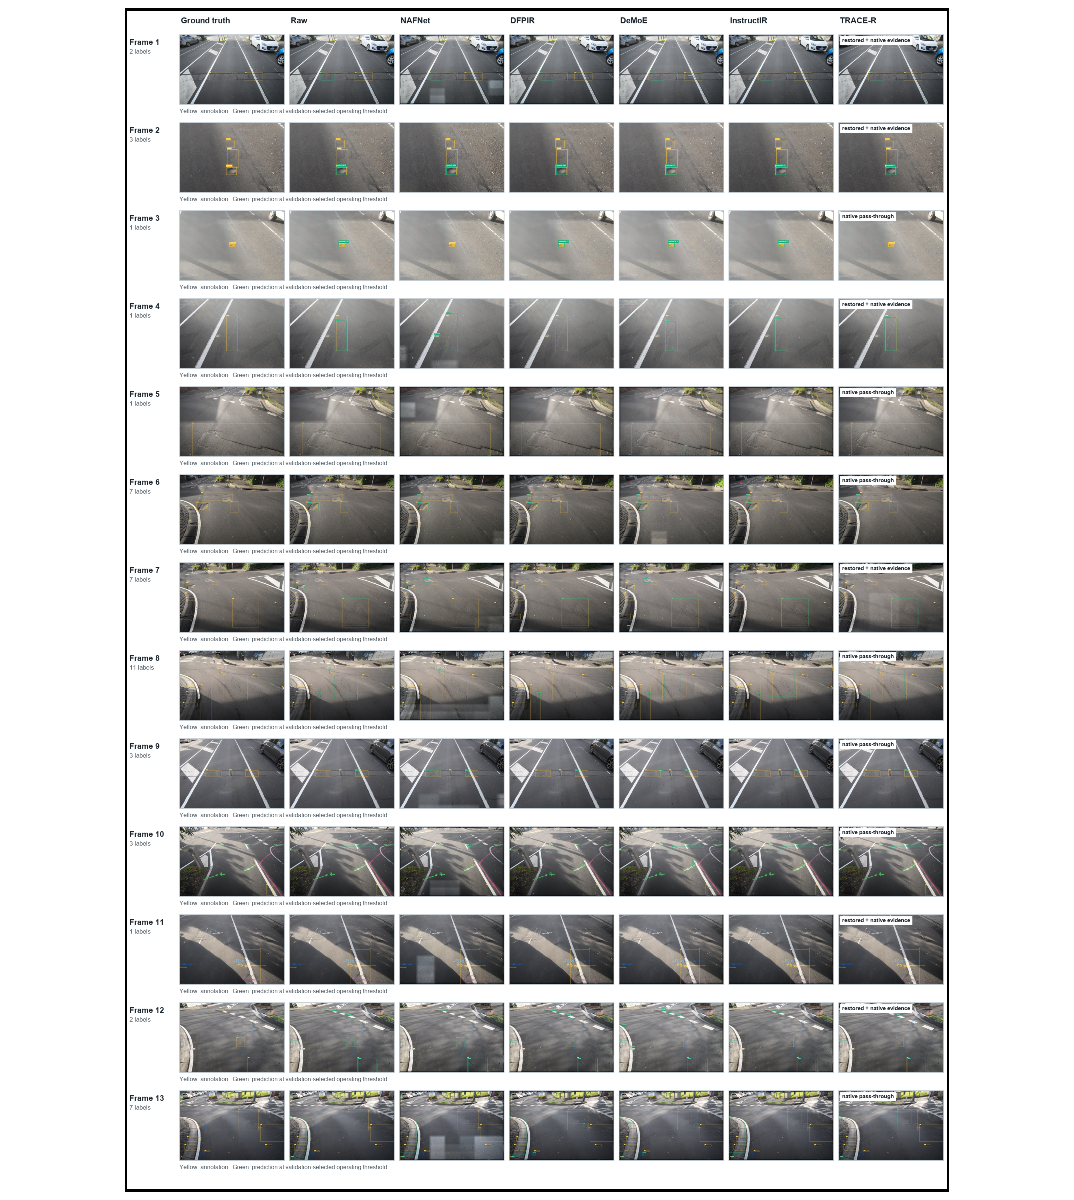
\includegraphics[width=\textwidth,height=0.82\textheight,keepaspectratio]{fig_trace_crid_all13.pdf}
\caption{All 13 CRID temporal-evaluation frames. Yellow boxes are annotations and green boxes are predictions at validation-fixed operating thresholds. TRACE-R labels each frame as native pass-through or native-plus-restored evidence.}
\label{fig:crid_all}
\end{figure*}

\section{Evidence and Reproducibility Boundaries}
The IVCNZ and PCM results are sequence/source-disjoint validation evidence. Earlier development opened the original test partitions, so those partitions are excluded from the reported claim. KITTI uses an earlier arXiv checkpoint. CRID uses a temporally earlier calibration segment and a non-overlapping but previously inspected evaluation segment. These boundaries are encoded in the provenance ledger and are not inferred from directory names.

The public release includes packet builders, matched training commands, expert-routing code, detector adapters, route constants, checkpoint hashes, qualitative-selection manifests, and the frozen result ledger. Historical file aliases remain only to reproduce old manifests. Paper-facing code and comments use TRACE-R, and all numerical tables in the manuscript are generated from the frozen ledger or the frozen CRID summaries.

\end{document}
